\newcommand{\tabitem}{~~\llap{\textbullet}~~}

\section{Functional Requirements}
To reach the main goals of the \emph{Travlendar+} application we need to satisfy these functional requirements:

\begin{requirementList}
	\item The user will have to specify a residence at registration time. This home address can be updated lately, thus the Software will have to permit to modify it. 
   
	\item The application must send a reminder to the user 30 minutes before he should begin the trip. Moreover, the application has to verify if a Sharing-Based vehicle is effectively available, if actually it is a user preference.
    
    \item If there isn't a Sharing based travel service available, the application must give a feasible alternative travel solution to the user according to his preferences.
    
    \item If two or more user's tasks have an overlapping, which cannot be schedule in a feasible way, the Application asks to the user to choose the task he prefers to do.
    
    \item The Software will have to permit the user to specify when he wants to return home. Thus, the software should have a special task representing it.
    
    \item The application has to reschedule a day if the user adds, deletes or updates a task during the day.
    
    \item If the user wants to add, delete or update a task during the day, the Application gives a travel solution that may not respect the time constraints.
    
    \item If the user adds a task that isn't reachable within the given time, the \emph{Travlendar+} System sends a warning to the user. 
    
    \item Each task can be repeated a finite or infinite number of times. In particular, a task can be repeated:
    \begin{enumerate}[label={[}R 9.\arabic*{]}:]
    \item the same day of every week
    \item the same day of every month
    \item the same day of every year
    \item two or more days during a single week
    \end{enumerate}
    Thus, the application should take care of repeated tasks considering the same specific preferences as defined by the user when creating the task.
    
    \item The application should consider whether the user is using private vehicles or not throughout a day.
    \begin{enumerate}[label={[}R 10.\arabic*{]}:]
    \item The Software should not suggest to use a private vehicle if the user left his residence without it.
   
    \item The software should consider that if the user left home using a private vehicle, it will be necessary to return home using the same private vehicle.
    \end{enumerate}
    
    \item The Software should permit to add or modify either general preferences, which are always taken care of, or specific preferences, which applies on a single task.
    \begin{enumerate}[label={[}R 11.\arabic*{]}:]
    \item If a specific preference conflicts with a general preference, the software will have to consider the specific one, ignoring the general one.
    \end{enumerate}
    
    \item The application should allow the user to insert tasks which are time-variable during the week. Thus, the Software should take care of these tasks scheduling them in an appropriate way, choosing day and time.
    
    \item The application should permit the purchase of either public transport service or vehicle sharing services through the respective external applications.
    
    \item The application should show all user's schedule with different kind of visualization: by month, by week or by day.
    
    \item The application should permit the selection of a single task, in order to show the relative preferences and should give the possibility to change these ones.
    
    \item The system has to guarantee new user signing up with a proper sign up page. 
    
    \item The system, in order to choose the best travel solution for the user, has to consider two main parameters: cost and time of the travel. To keep this kind of information, the system uses this formula: \( y = a \cdot cost + b \cdot time\). Therefore, the system will minimize the \(y\) variable. If there is two kinds of travels which have the same \(y\) value, so the application will ask to the user.
    
    \item If public transport is a user's preference, the system has to suggest the best ticket available with respect to the user's tasks. 
    \begin{enumerate}[label={[}R 18.\arabic*{]}:]
    \item If the user has already a season ticket, then this information will be taken into account when scheduling new and old user's tasks.
    \end{enumerate}

\end{requirementList}

\section{Use Case Diagram and Scenarios description}
\subsection{Login System}
Every user who wants to use the \emph{Travlendar+} application should be registered to the application System.
After that, the user has to log in into our System in order to be recognized and to see his personal calendar.

\begin{table}[H]
	\centering
    
    \begin{tabular}{|p{3.5cm}|p{10.3cm}|}
    
    \hline
    \textbf{\large{Actors}}  			& \tabitem Visitor 									\\
    				 					& \tabitem Registered User							\\
                     					& \tabitem Logged-In User 							\\
    \hline
    \textbf{\large{Goals}} 				& \ref{goal:login} 									\\
    
    \hline
    \textbf{\large{Enter Condition}}	& There is no enter condition for this Use Case		\\
    
    \hline
    \textbf{\large{Events Flow}}		& \begin{enumerate}[leftmargin=0.5cm]
                                          	\item The \emph{Visitor}  access to the web site or application log in page
                                            \item The \emph{Visitor} fills all the mandatory information (personal data, password, email)
                                            \item The \emph{Travlendar+} System registers the user and send back a confirmation email
                                            \item The \emph{Visitor} user becomes a \emph{Registered} user inserting his email and password in the log in page   
                                            \item The \emph{Registered} user now can access the \emph{Travlendar+} services through the log in page
                                            
                                            \item After the insertion of username and password, the user becomes a \emph{Logged in} user
                                          \end{enumerate}
    										\\
    \hline
    \textbf{\large{Exit Condition}} 	& The user is registered in the \emph{Travlendar+} System, and his account is created. Now the user is able to access to his 													calendar and his account through both the web site and the mobile application \\
    
    \hline
    \textbf{\large{Exception}} 			& The \emph{Visitor} is not able to register himself because is already registered.\newline The \emph{Registered} user                                         is not able to sign in the System because the inserted username or password are wrong or if he did not confirmed                                           his email. \newline
    										All these kind of exceptions will be handled by the System showing to the user an error message either in the website or in the mobile application \\
    
    \hline
    
    
    \end{tabular}
	
\end{table}

\begin{figure}[H]
\centering
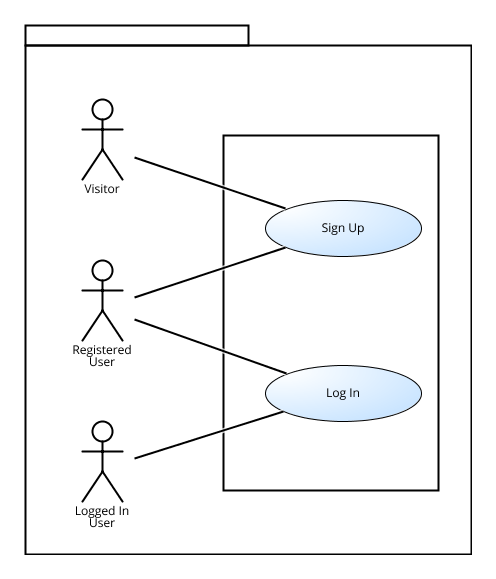
\includegraphics[scale=0.5]{Pictures/UseCaseDiagram/Log_In_System.png}
\caption{UML Use Case Diagram for Log In System}
\end{figure}

\begin{figure}[H]
\centering
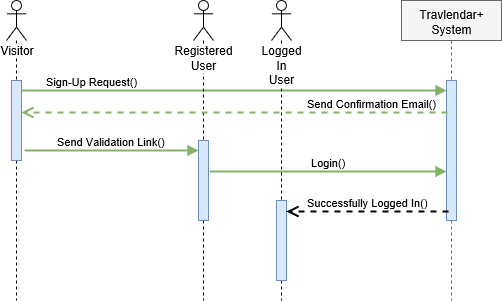
\includegraphics[scale=0.5]{Pictures/SequenceDiagram/login.png}
\caption{UML Sequence Diagram for Log In System}
\end{figure}

From this point among the next sections, we consider as the \emph{User} a logged user.
\subsection{Adding a new Task}
In this section is reported the procedure used to create and add a new task to the user's calendar.
The user can select a variety of preferences to adapt the task to his needs, indeed he can select when and where the task will take place, how he wants to reach the location of that task, the task priority and the maximum walk range. In this way our System will be able to schedule the user's calendar according to both the user preferences and the task preferences, giving more priority to the latter. If an overlap occurs or if a certain task is unreachable the System will notify the user asking respectively to choose from one of the overlapping tasks or to change some task setting. At this purpose, see the Sequence Diagram below that models this situation.     

Notice that, there are some preferences which are mandatory (the ones listed below under the Events Flow voice) while other are not, thus, default values will be automatically set by the System. In addition, we must highlight that the Events Flow voices from point 2 to 5 might be executed by the user as he prefers.

\begin{table}[H]
	\centering
    
    \begin{tabular}{|p{3.5cm}|p{10.3cm}|}
    
    \hline
    \textbf{\large{Actors}}  			& \tabitem User\\
    
    \hline
    \textbf{\large{Goals}} 				& \ref{goal:task}; \ref{goal:taskBehavior}; \ref{goal:noTaskConflict}; \ref{goal:impossibleTask}; \ref{goal:priority}; \ref{goal:retakeCar}\\
    
    \hline
    \textbf{\large{Enter Condition}}	& The user should log in the \emph{Travlendar+} System and he 												is on the calendar page\\
    
    \hline
    \textbf{\large{Events Flow}}		& \begin{enumerate}[leftmargin=0.5cm]
                                          	\item The user press on the \emph{"Add a new Task"} button
                                            \item The user select at least one \emph{time} preference
                                            \item The user select at least one \emph{day} preference
                                            \item The user insert a location, where the task will take place
                                            \item The user select if the task has to be a periodic task 														or not. If the task has a periodicity, the user has to 															select when the task should be repeated
                                            \item The user can select other elective options, for instance the priority of the task, the maximum walk range or a preferred vehicle to reach the task. If the user skips this phase, then automatically default preferences will be applied
                                            \item The user confirm the task just created
                                          \end{enumerate}
    										\\
    \hline
    \textbf{\large{Exit Condition}} 	& The task just created by the user is successfully added to the user's 											schedule\\
    
    \hline
    \textbf{\large{Exception}} 			& The task just created by the user is not added to the calendar. It may be happen either for an overlapping (e.g this task's time slot is overlapped with another task that is already in the calendar) or for some wrong information inserted in the creation phase. For the former problem, the user has to select which task he prefers, for the latter the user has to create again the task inserting the correct information \\
    
    \hline
    
    
    \end{tabular}
	
\end{table}

\begin{figure}[H]
\centering
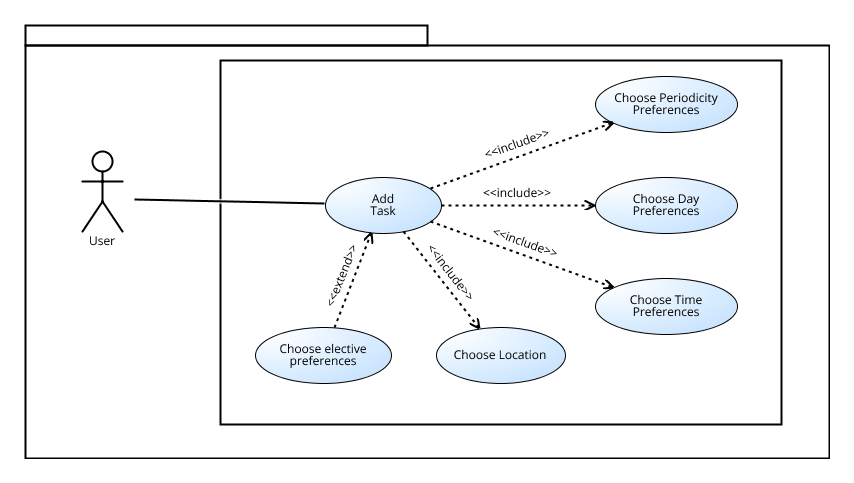
\includegraphics[scale=0.5]{Pictures/UseCaseDiagram/Adding_a_new_task.png}
\caption{UML Use Case Diagram for the addition of a new task }
\end{figure}

\begin{figure}[H]
\centering
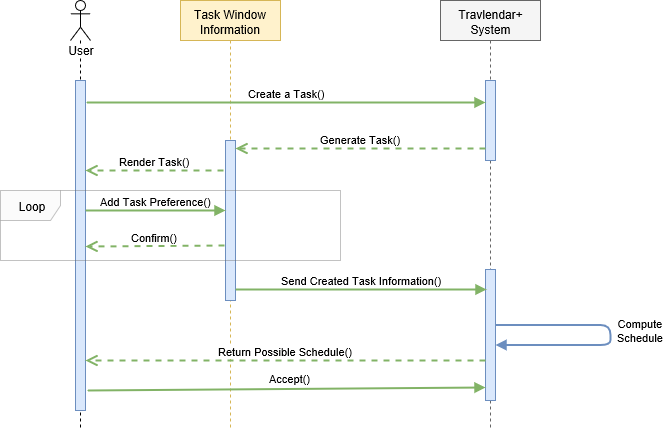
\includegraphics[scale=0.5]{Pictures/SequenceDiagram/adding_a_task.png}
\caption{UML Sequence Diagram for the addition of a new task, \emph{without overlapping}}
\end{figure}

\begin{figure}[H]
\centering
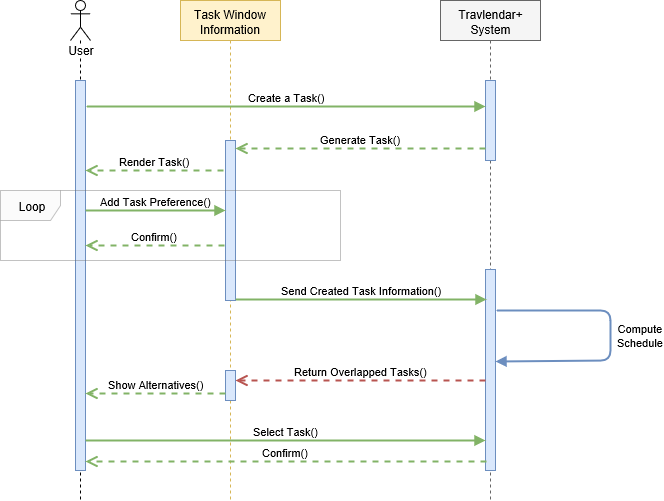
\includegraphics[scale=0.5]{Pictures/SequenceDiagram/adding_a_task_with_overlapping.png}
\caption{UML Sequence Diagram for the addition of a new task, \emph{with overlapping}}
\end{figure}
\subsection{Modify an existing task}

It may happen that the user wants to modify an existing task since his travel mean preferences are changed or the appointment time or location are changed. It can also be the case that the user wants to delete a scheduled appointment. These features are described in this section.

\begin{table}[H]
	\centering
    
    \begin{tabular}{|p{3.5cm}|p{10.3cm}|}
    
    \hline
    \textbf{\large{Actors}}  			& \tabitem User\\
    
    \hline
    \textbf{\large{Goals}} 				& \ref{goal:task}; \ref{goal:taskBehavior}; \ref{goal:preferences}; \ref{goal:retakeCar}\\
    
    \hline
    \textbf{\large{Enter Condition}}	& The user should be logged in the                                                        \emph{Travlendar+} System\\
    
    \hline
    \textbf{\large{Events Flow}}		& \begin{enumerate}[leftmargin=0.5cm]
                                             
                                          	\item The user select the task he wants to change from his calendar (doing this he can also change the time scope of the calendar: daily, weekly, monthly time scope)
                                          	\item Now he can decide to modify some preferences, such as the time, the date, the location or the priority of the selected task. Moreover, the user can choose to cancel the entire task
                                          	\item The user confirm to apply the changes or discard them
                                          	\item The \emph{Travlendar+} System computes a new schedule according to the new user preferences
                                          	\item Finally the user can choose from the new calendar or the older one
                                          \end{enumerate}
    										\\
    \hline
    \textbf{\large{Exit Condition}} 	& The user has chosen which calendar he prefers:                                          the newer or the older; So, from now on, the System will behave accordingly to the updated calendar\\
    
    \hline
    \textbf{\large{Exception}} 			& The modification of the task is not valid, for instance the user has inserted some wrong information about the task, then the user has to modify the task again. \newline
    The modification of the task has created an overlap with another task, so the user has to choose which task he prefers to have in his calendar.\\
    
    \hline
    
    
    \end{tabular}
	
\end{table}

\begin{figure}[H]
\centering
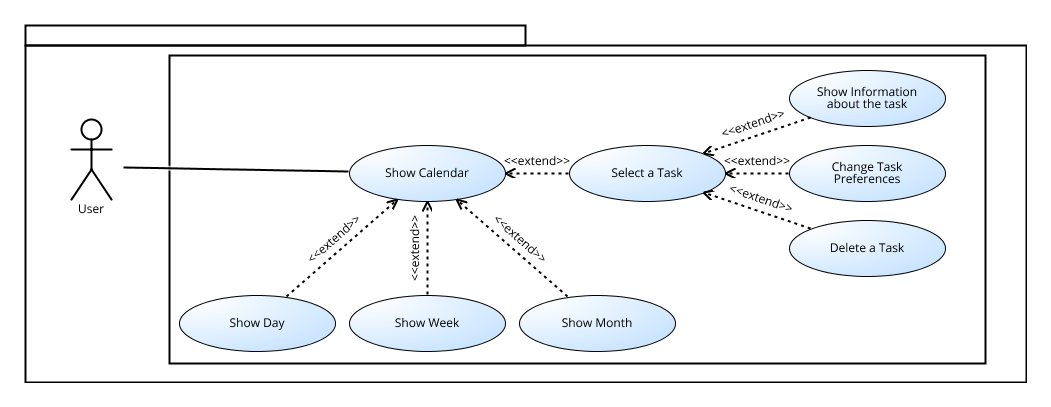
\includegraphics[scale=0.5]{Pictures/UseCaseDiagram/Rescheduling.png}
\caption{UML Use Case Diagram for the modification of a new task and the rescheduling of the calendar}
\end{figure}

\begin{figure}[H]
\centering
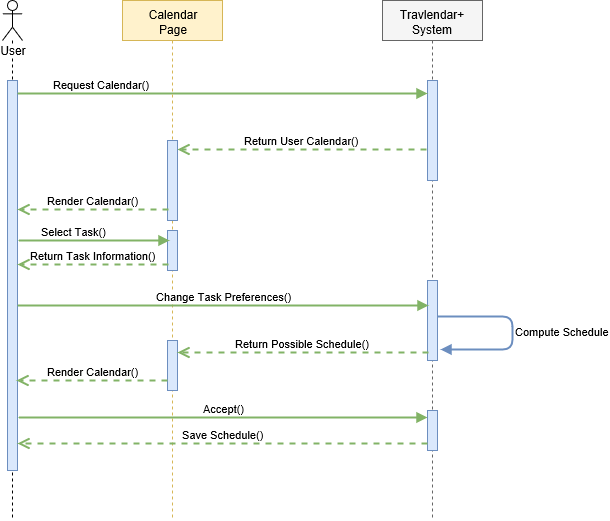
\includegraphics[scale=0.5]{Pictures/SequenceDiagram/rescheduling.png}
\caption{UML Sequence for the modification of a new task and the rescheduling of the calendar}
\end{figure}
\subsection{Adding a break time}
In the \emph{Travlendar+} application if the user wants to have some free time he can create a break time. For instance, if the user wants to have lunch at 1 p.m. he can add to his calendar a break time task. This particular kind of task is scheduled according to the user's preferences as a normal task, with flexible time and periodicity but, without a specific location: we suppose that the user will have a break close to where he is.
In addition, if the break time is scheduled close to lunch time, then the \emph{Travlendar+} System will suggest the user a place where to eat.


\begin{table}[H]
	\centering
    
    \begin{tabular}{|p{3.5cm}|p{10.3cm}|}
    
    \hline
    \textbf{\large{Actors}}  			& \tabitem User\\
    
    \hline
    \textbf{\large{Goals}} 				& \ref{goal:task}; \ref{goal:breakTask}; \ref{goal:taskBehavior}; \ref{goal:preferences}; \ref{goal:retakeCar}\\
    
    \hline
    \textbf{\large{Enter Condition}}	& The user should be logged in the                                                        \emph{Travlendar+} system\\
    
    \hline
    \textbf{\large{Events Flow}}		& \begin{enumerate}[leftmargin=0.5cm]
                                          	\item The user presses the "Add a FixedTask" button
                                          	\item The user select "Break Time" as task preferences
                                          	\item The user insert some additional information about the task, such as the time when he wants to do that break
                                          	\item The user select the repetition of that break time task
                                          	\item The user should approve or discard the task
                                          	\item Finally the system compute a schedule according the user's preferences and the break time just inserted
                                          \end{enumerate}
    										\\
    \hline
    \textbf{\large{Exit Condition}} 	& The user either accept the proposed schedule or discard it\\
    
    \hline
    \textbf{\large{Exception}} 			& The break time just inserted is overlapped with other tasks                                         yet inserted in the user's calendar, so the user should                                           select another break time or cancel the other task\\
    
    \hline
    
    
    \end{tabular}
	
\end{table}

\begin{figure}[H]
\centering
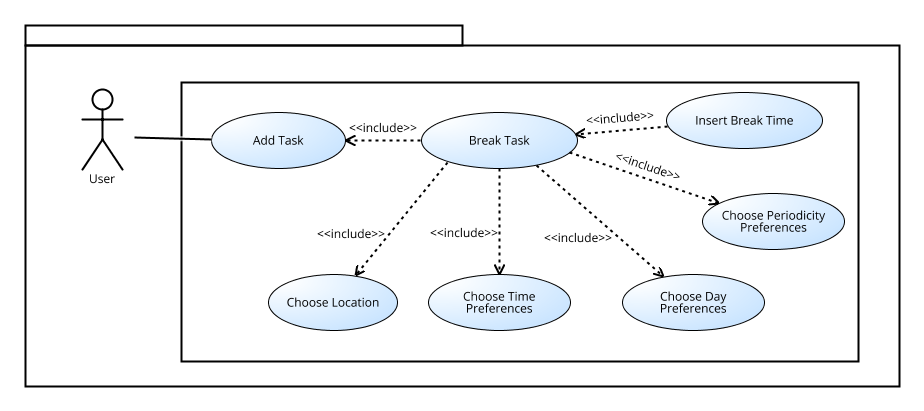
\includegraphics[scale=0.5]{Pictures/UseCaseDiagram/Add_a_break_time.png}
\caption{UML Use Case Diagram for the addition of a break time task }
\end{figure}

\subsection{Show Transport Information about a FixedTask}

If the user wants more information about what kind of vehicles he needs to take to reach others tasks location, he can select a task from the calendar page and automatically more information about that task will be shown. For example, the trip indications and the travel means involved: if he needs to take a bus, a share-based vehicle or his own vehicle. Notice that, if the user take his own private vehicle, the application will schedule the day travels in such a way that allows the user to retake his own vehicle. 

\begin{table}[H]
	\centering
    
    \begin{tabular}{|p{3.5cm}|p{10.3cm}|}
    
    \hline
    \textbf{\large{Actors}}  			& \tabitem User\\
    
    \hline
    \textbf{\large{Goals}} 				& \ref{goal:travel}; \ref{goal:retakeCar}\\
    
    \hline
    \textbf{\large{Enter Condition}}	& The user should be logged in the                                                                    \emph{Travlendar+} system and there is a calendar that is                                         just scheduled\\
    
    \hline
    \textbf{\large{Events Flow}}		& \begin{enumerate}[leftmargin=0.5cm]
                                          	\item The user select a task from his calendar
                                          	\item The user presses the "Show Transport Information" button on the task menu
                                          	\item Now the user can choose from different kind of information: the vehicle he should take, the road trip he should do or the instructions to reach that location
                                          	\item Finally the user can look at the information he needs about transport systems
                                          \end{enumerate}
    										\\
    \hline
    \textbf{\large{Exit Condition}} 	& The user closes the \emph{Transport Information} screen and return to the \emph{Calendar} page\\
    
    \hline
    \textbf{\large{Exception}} 			& \\
    
    \hline
    
    
    \end{tabular}
	
\end{table}

\begin{figure}[H]
\centering
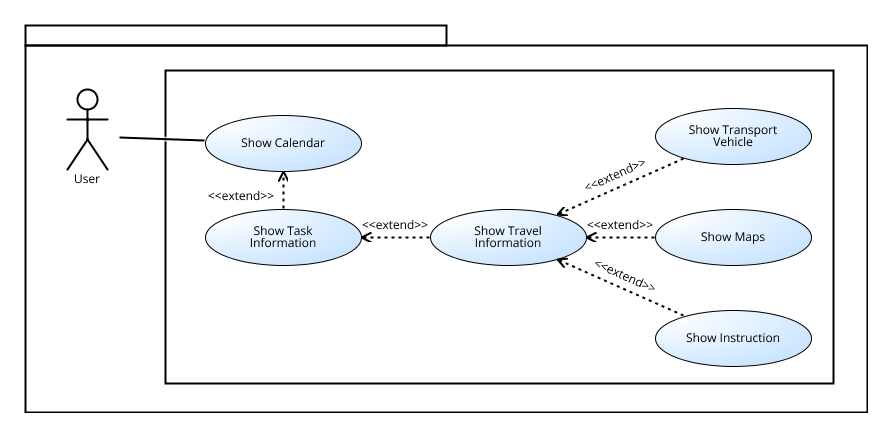
\includegraphics[scale=0.5]{Pictures/UseCaseDiagram/Transport_Instruction.png}
\caption{UML Use Case Diagram for the transport information about a task}
\end{figure}
\subsection{Buying a vehicle-sharing or a public transport service}
The user, for some tasks, maybe wants to take a bus or another public transport service. Furthermore, in Milan there are lots of alternatives to public transport, such as the car-sharing or the bike-sharing services, so the user might want to use one of these to reach a task location. For this reason, the \emph{Travlendar+} System, not only support the user in the process of choosing and buying a possible ticket from the public transport site or application, but also redirects the user to the right place where to book and rent a shared based travel mean service.

\begin{table}[H]
	\centering
    
    \begin{tabular}{|p{3.5cm}|p{10.3cm}|}
    
    \hline
    \textbf{\large{Actors}}  			& \tabitem User\\
                                        & \tabitem Car-Sharing Service\\
                                        & \tabitem Bike-Sharing Service\\
                                        & \tabitem Public Transport Service\\
                                        
    \hline
    \textbf{\large{Goals}} 				& \ref{goal:travel} \ref{goal:buyTicket}\\
    
    \hline
    \textbf{\large{Enter Condition}}	& The user should be logged in the                                                        \emph{Travlendar+} system and the calendar should be already scheduled\\
    
    \hline
    \textbf{\large{Events Flow}}		& \begin{enumerate}[leftmargin=0.5cm]
                                          	\item The user select a task
                                          	\item The user press the "Show Transport Information" button
                                          	\item The user select the type of transport service he wants to use
                                          	\item The user then selects if he wants to buy the ticket
                                          \end{enumerate}
    										\\
    \hline
    \textbf{\large{Exit Condition}} 	& The user should confirm the operation, then the system redirects he to the correct site of the selected service: Car-Sharing, Bike-Sharing or Public Transport\\
    
    \hline
    \textbf{\large{Exception}} 			& \\
    
    \hline
    
    
    \end{tabular}
	
\end{table}

\begin{figure}[H]
\centering
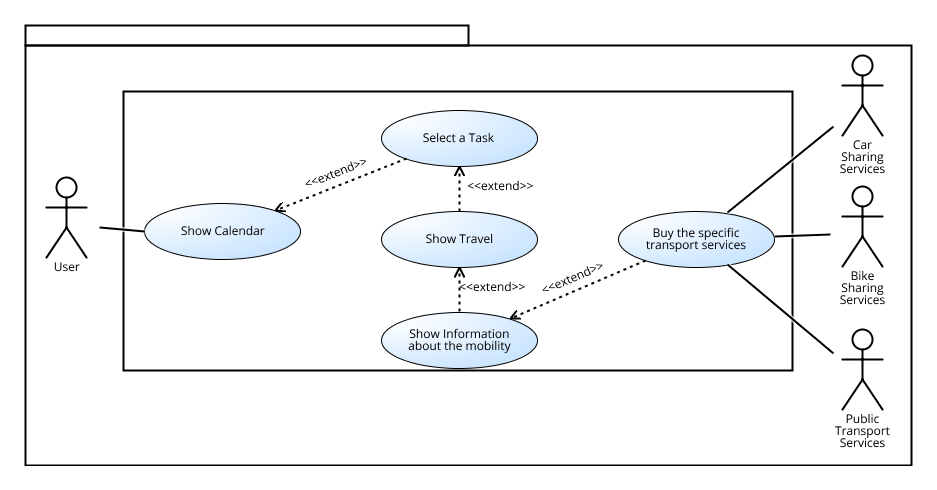
\includegraphics[scale=0.5]{Pictures/UseCaseDiagram/Buy_services.png}
\caption{UML Use Case Diagram for buying services operation DA RENDERE COERENTE CON SHOW TRANSPORT INFO: SHOW CAL, SHOW TASK, SHOW TRAV INFO... VEDI ANCHE UML DI MODIFY TASK: CHANGE TASK PREF E SHOW INFO}
\end{figure}

\subsection{Reminder System}
A nice feature provided by the \emph{Travlendar+} System is that it is possible to access the System either on traditional computer (through a web browser) or on a mobile phone (through the mobile application). 

In both cases, the user may want to receive a notification that suggest him to start his travel, in order to reach the location of the next task. Moreover, it may happen that the user wants to take a vehicle-shared based service, but in the very moment he starts his trip, there isn't a vehicle available. To overcome these issues, the \emph{Travlendar+} System sends a reminder to the user, and if the user wants to take a vehicle-shared based service, our System, 30 minutes before the trip starts, will check if there are vehicles available, and suggest to the user to book that vehicle.

\begin{figure}[H]
\centering
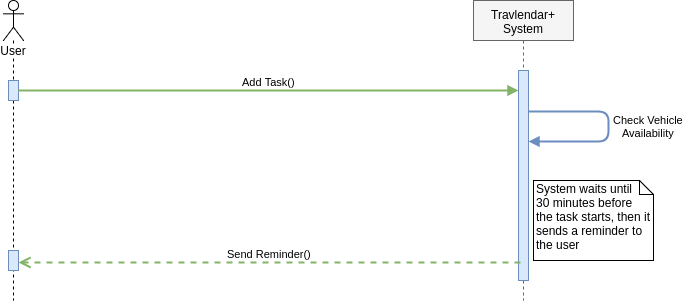
\includegraphics[scale=0.5]{Pictures/SequenceDiagram/reminder.png}
\caption{UML Sequence Diagram for the Reminder Notification System}
\end{figure}
\subsection{Asking information about Public Transport Service}
The \emph{Travelndar+} System will interact with the Public Transport system, to suggest the best ticket option in terms of money, time and considering the user agenda.

Several times public transport service is unavailable for many reasons, for instance an incoming strike or a maybe some metro line are stopped because of maintenance. Also in such situations the user wants to reach his appointments in time, and so the \emph{Travlendar+} System should retrieve this information from the Public Transport system, to properly schedule the user's calendar. 

\begin{table}[H]
	\centering
    
    \begin{tabular}{|p{3.5cm}|p{10.3cm}|}
    
    \hline
    \textbf{\large{Actors}}  			& \tabitem Public Transport System\\
    
    \hline
    \textbf{\large{Goals}} 				& \ref{goal:task}; \ref{goal:reachability}; \ref{goal:travel}; \ref{goal:travel}; \ref{goal:purchase} \\
    
    \hline
    \textbf{\large{Enter Condition}}	& The \emph{Travlendar+} system starts to schedule the user's calendar\\
    
    \hline
    \textbf{\large{Events Flow}}		& \begin{enumerate}[leftmargin=0.5cm]
                                          	\item The \emph{Travlendar+} System asks mobility information or travel cards information to the \emph{Public Transport} system through existing APIs
                                          	\item The \emph{Public Transport} system sends back all the required information that the \emph{Travlendar+} service has requested
                                          \end{enumerate}
    										\\
    \hline
    \textbf{\large{Exit Condition}} 	& The \emph{Travlendar+} system has requested all the mobility information it needed from the \emph{Public Transport} service\\
    
    \hline
    \textbf{\large{Exception}} 			& It can be happened that either the \emph{Public Transport} service is unavailable or an information request is rejected. In the former case it is impossible knowing useful information in order to schedule the user's calendar, so the \emph{Travlendar+} system will compute a calendar without those information; otherwise in the latter case our system tries to ask again the information it needs\\
    
    \hline
    
    
    \end{tabular}
	
\end{table}

\begin{figure}[H]
\centering
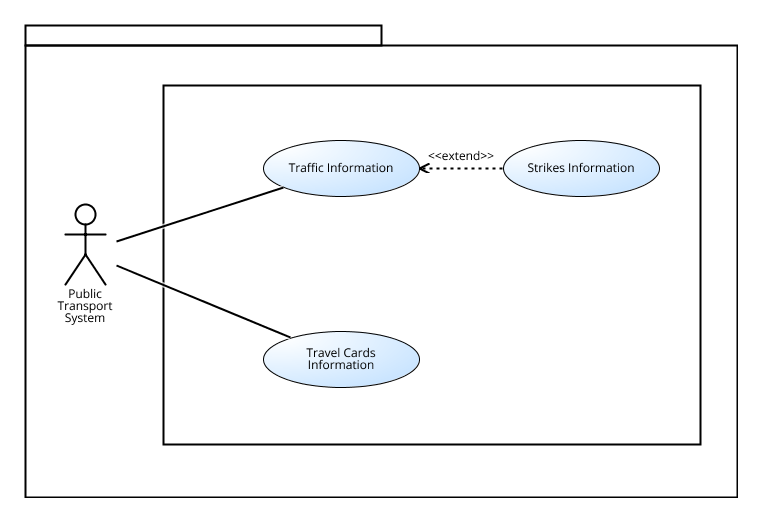
\includegraphics[scale=0.5]{Pictures/UseCaseDiagram/ATM.png}
\caption{UML Use Case Diagram for the information requests asked to the \emph{Public Transport} service}
\end{figure}
\subsection{Using external Maps Services}
In order to compute, as well as possible, the user's calendar, the \emph{Travlendar+} service needs to know more information about the status of interested roads, the traffic information about the city and other useful information concerning the user's trip.
To reach this goal the \emph{Travlendar+} System needs to interact with an external maps service, retrieving these kind of information.

\begin{table}[H]
	\centering
    
    \begin{tabular}{|p{3.5cm}|p{10.3cm}|}
    
    \hline
    \textbf{\large{Actors}}  			& \tabitem External Maps Service\\
    
    \hline
    \textbf{\large{Goals}} 				& \ref{goal:task}; \ref{goal:reachability}; \ref{goal:timeslot}; \ref{goal:travel}; \ref{goal:piotti}\\
    
    \hline
    \textbf{\large{Enter Condition}}	& The \emph{Travlendar+} service is computing the user's calendar, so it needs to know more information about the user's trip\\
    
    \hline
    \textbf{\large{Events Flow}}		& \begin{enumerate}[leftmargin=0.5cm]
                                          	\item The \emph{Travlendar+} system asks the maps information to the \emph{External Maps} service through APIs
                                          	\item The \emph{External Maps} service sends back the maps information
                                          	\item The \emph{Travlendar+} now asks to the \emph{External Maps} service to compute a trip
                                          	\item The \emph{External Maps} service finally sends back the road trip just computed and more useful information about that journey
                                          \end{enumerate}
    										\\
    \hline
    \textbf{\large{Exit Condition}} 	& The \emph{Travlendar+} service knows all the information it needs in order to schedule as well as possible the user's calendar\\
    
    \hline
    \textbf{\large{Exception}} 			& It may be happened that the \emph{External Maps} is unavailable for some reasons, in this case the \emph{Travlendar+} system cannot compute the user's calendar, and our system tries to schedule it later with another request to the maps service\\
    
    \hline
    
    
    \end{tabular}
	
\end{table}

\begin{figure}[H]
\centering
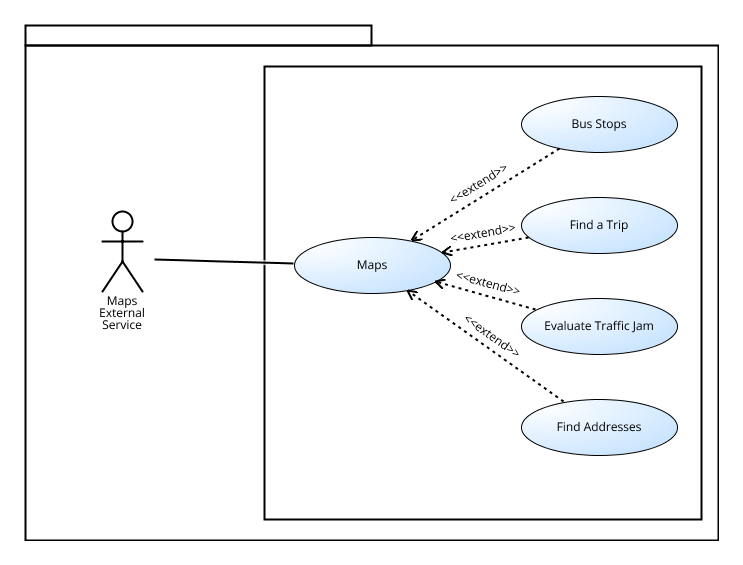
\includegraphics[scale=0.5]{Pictures/UseCaseDiagram/Google.png}
\caption{UML Use Case Diagram for the information requests about the maps}
\end{figure}